% !TEX root = ./document.tex

\documentclass[a4paper, spanish]{article}

\usepackage{mystyle}
\usepackage{myvars}

\begin{document}

  \maketitle

  \begin{itemize}
    \item \textbf{Archivo}: \texttt{weight-loss.csv}
    \item \textbf{Serie}: Frecuencia de búsquedas para la palabra clave \say{Weight loss} a través del buscador \emph{Google} por meses, desde \emph{Enero de 2004} hasta \emph{Diciembre de 2018}. Los valores han sido estandarizados en el rango $[0, 100]$.
  \end{itemize}

  \section{Etapa de identificación}
  \label{sec:1}

    \paragraph{}
    Tal y como se indica al comienzo de este documento, en este trabajo se va a trabajar con la serie temporal referida a la frecuencia de búsqueda de la palabra clave \say{Weight loss} (a nivel mundial) a través del buscador \emph{Google}. Se ha escogido esta serie para el trabajo por su estructura estacional claramente marcada. Se cree que dicha estructura tiene un alto grado de relación con un índice sobre la preocupación de la población por su peso a lo largo del tiempo.

    \paragraph{}
    Para evitar problemas de privacidad, los datos se proporcionan estandarizados en el rango $[0, 100]$, lo cual elimina la escala de los mismos y únicamente permite estudiar la estructura estocástica de la serie. Esto no es un problema para el análisis que se realizará en este trabajo, dado que precisamente el objetivo del mismo es el de analizar la estructura de una serie serie temporal, siguiendo la metodología de \emph{Box-Jenkins}.

    \paragraph{}
    En cuanto al particionamiento de los datos, estos se proporcionan en agrupaciones mensuales. Dado que se tiene información desde \emph{Enero de 2004} hasta \emph{Diciembre de 2018}, es decir, un total de \emph{15 años}, lo cual suma $15 * 12 = 180$ observaciones en total. Con esta cantidad de observaciones, se cree que se podrá construir un modelo \emph{SARIMA} (\emph{ARIMA} con estacionalidad) de manera adecuada.

    \begin{figure}
      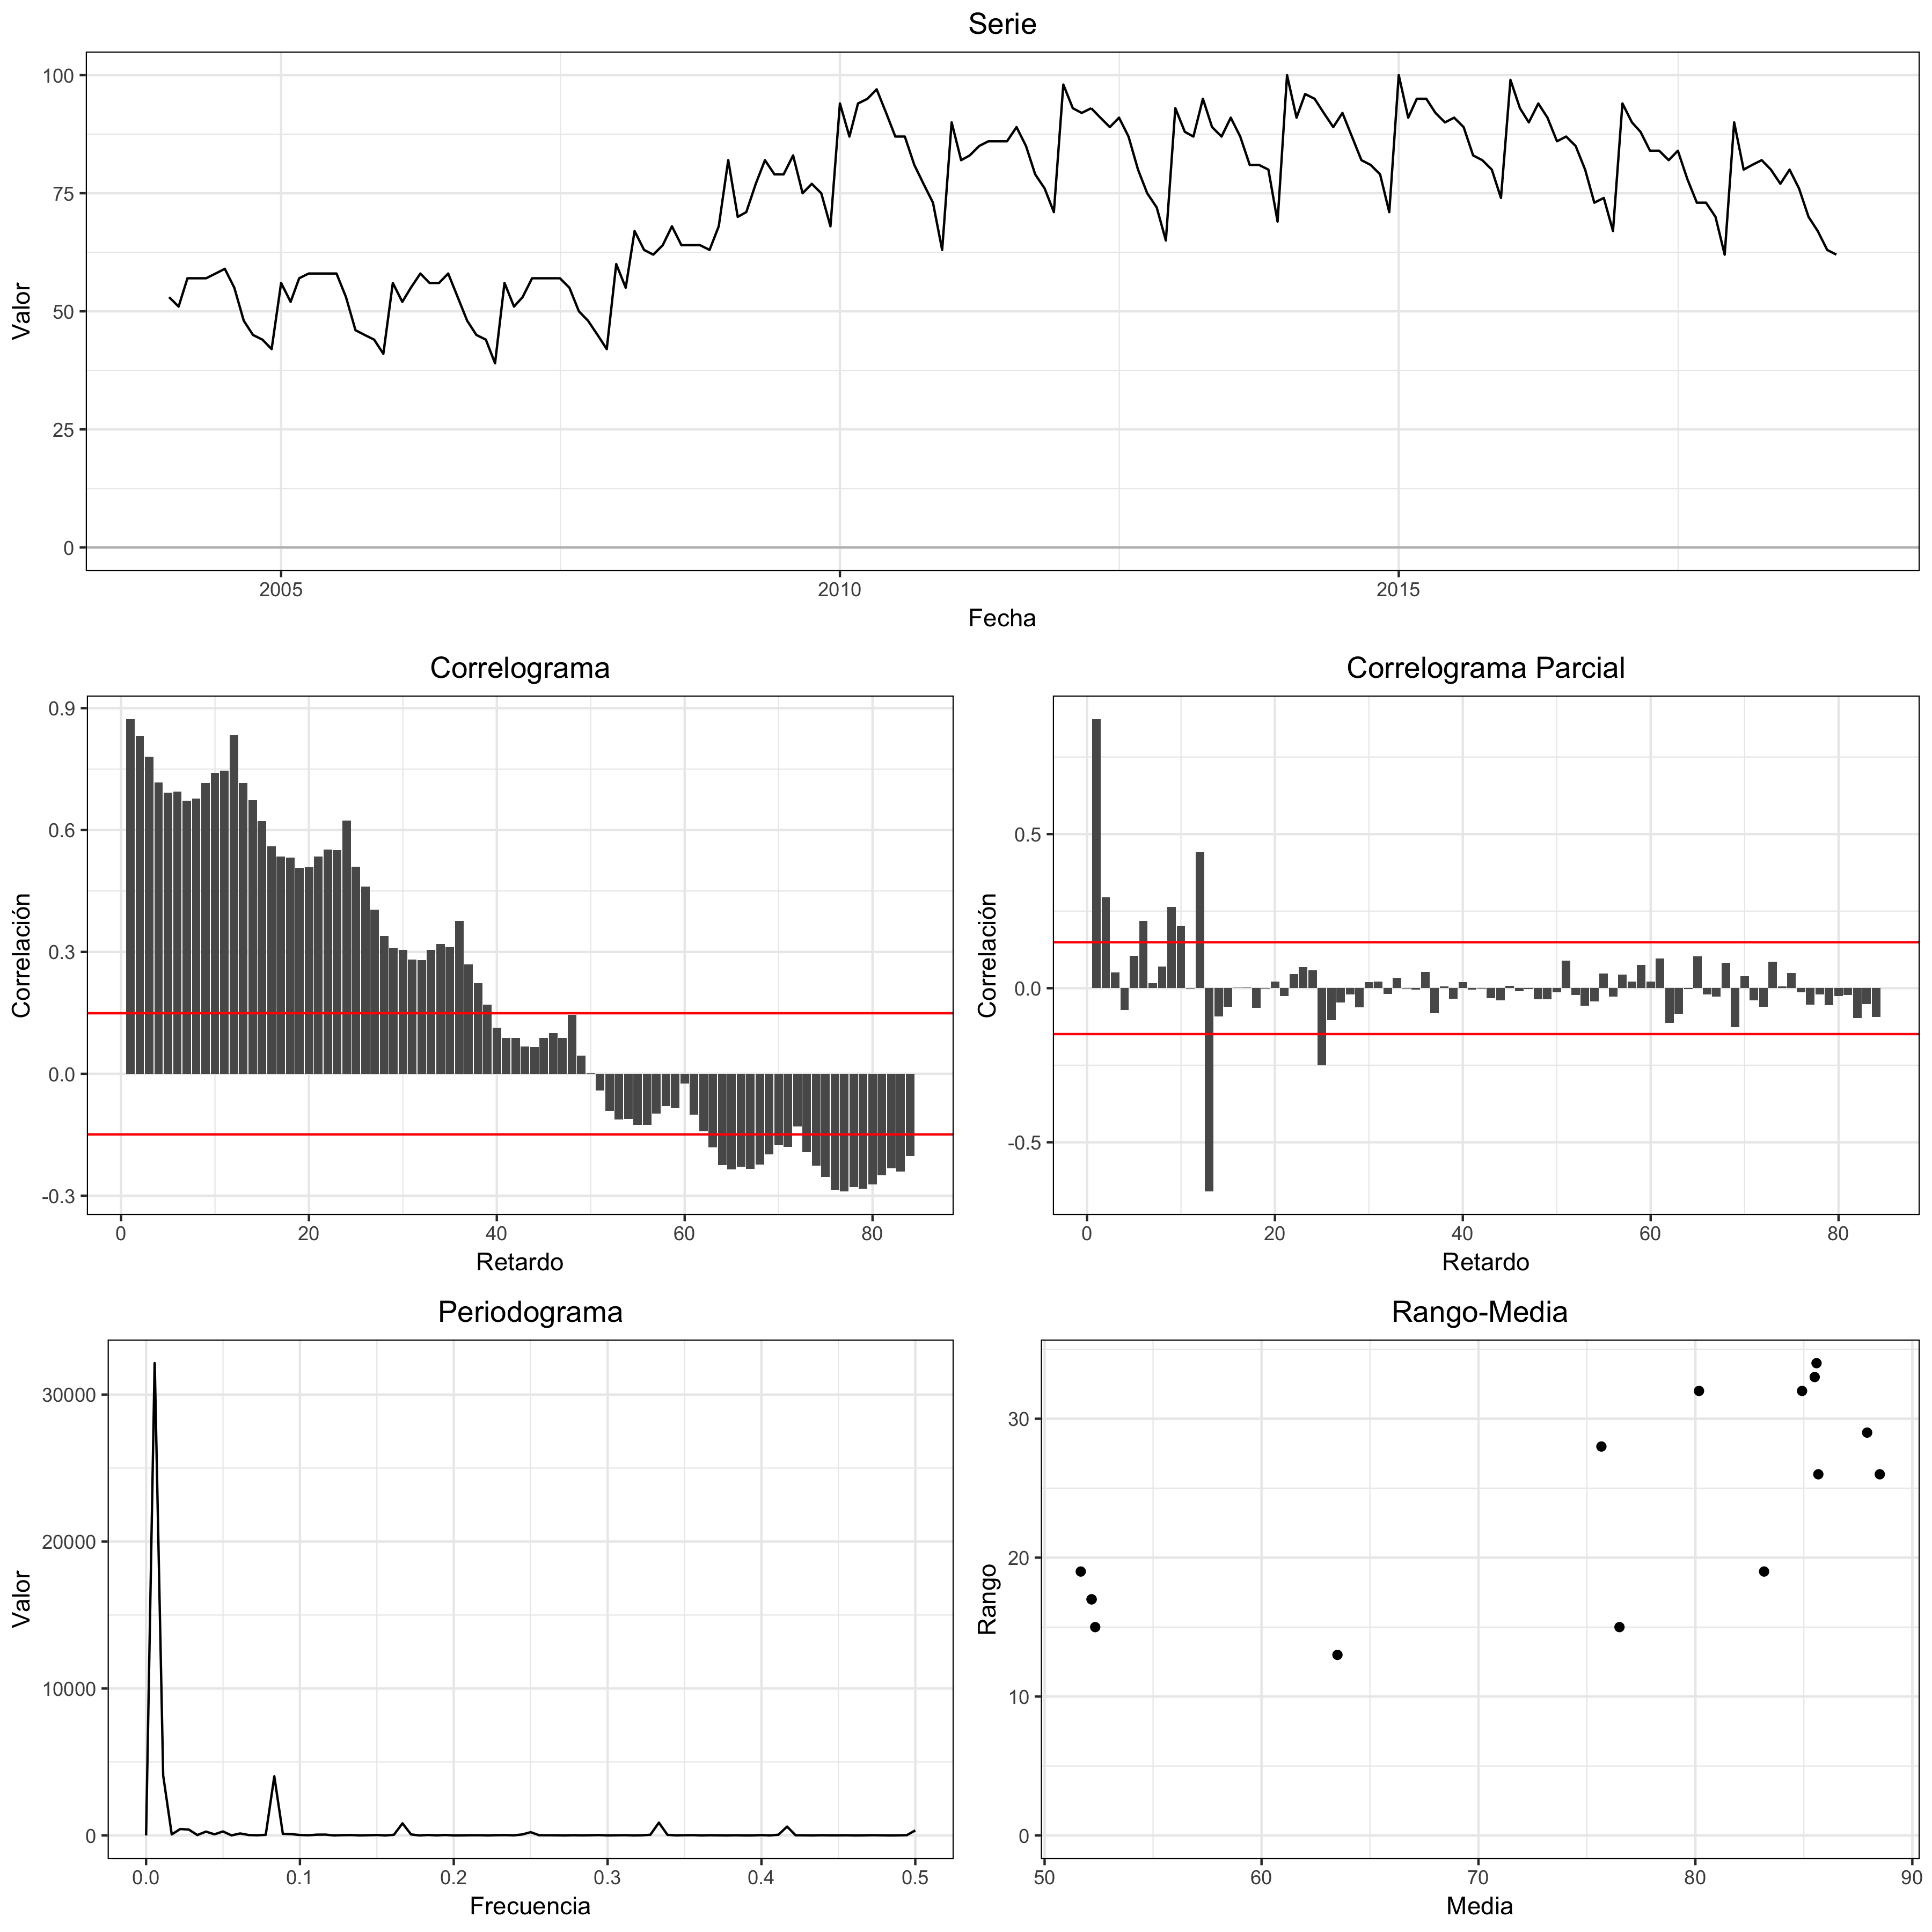
\includegraphics[width=\textwidth,height=\textheight,keepaspectratio]{weightloss}
      \caption{[TODO]}
      \label{}
    \end{figure}

    \paragraph{}
    [TODO]

    \begin{figure}
      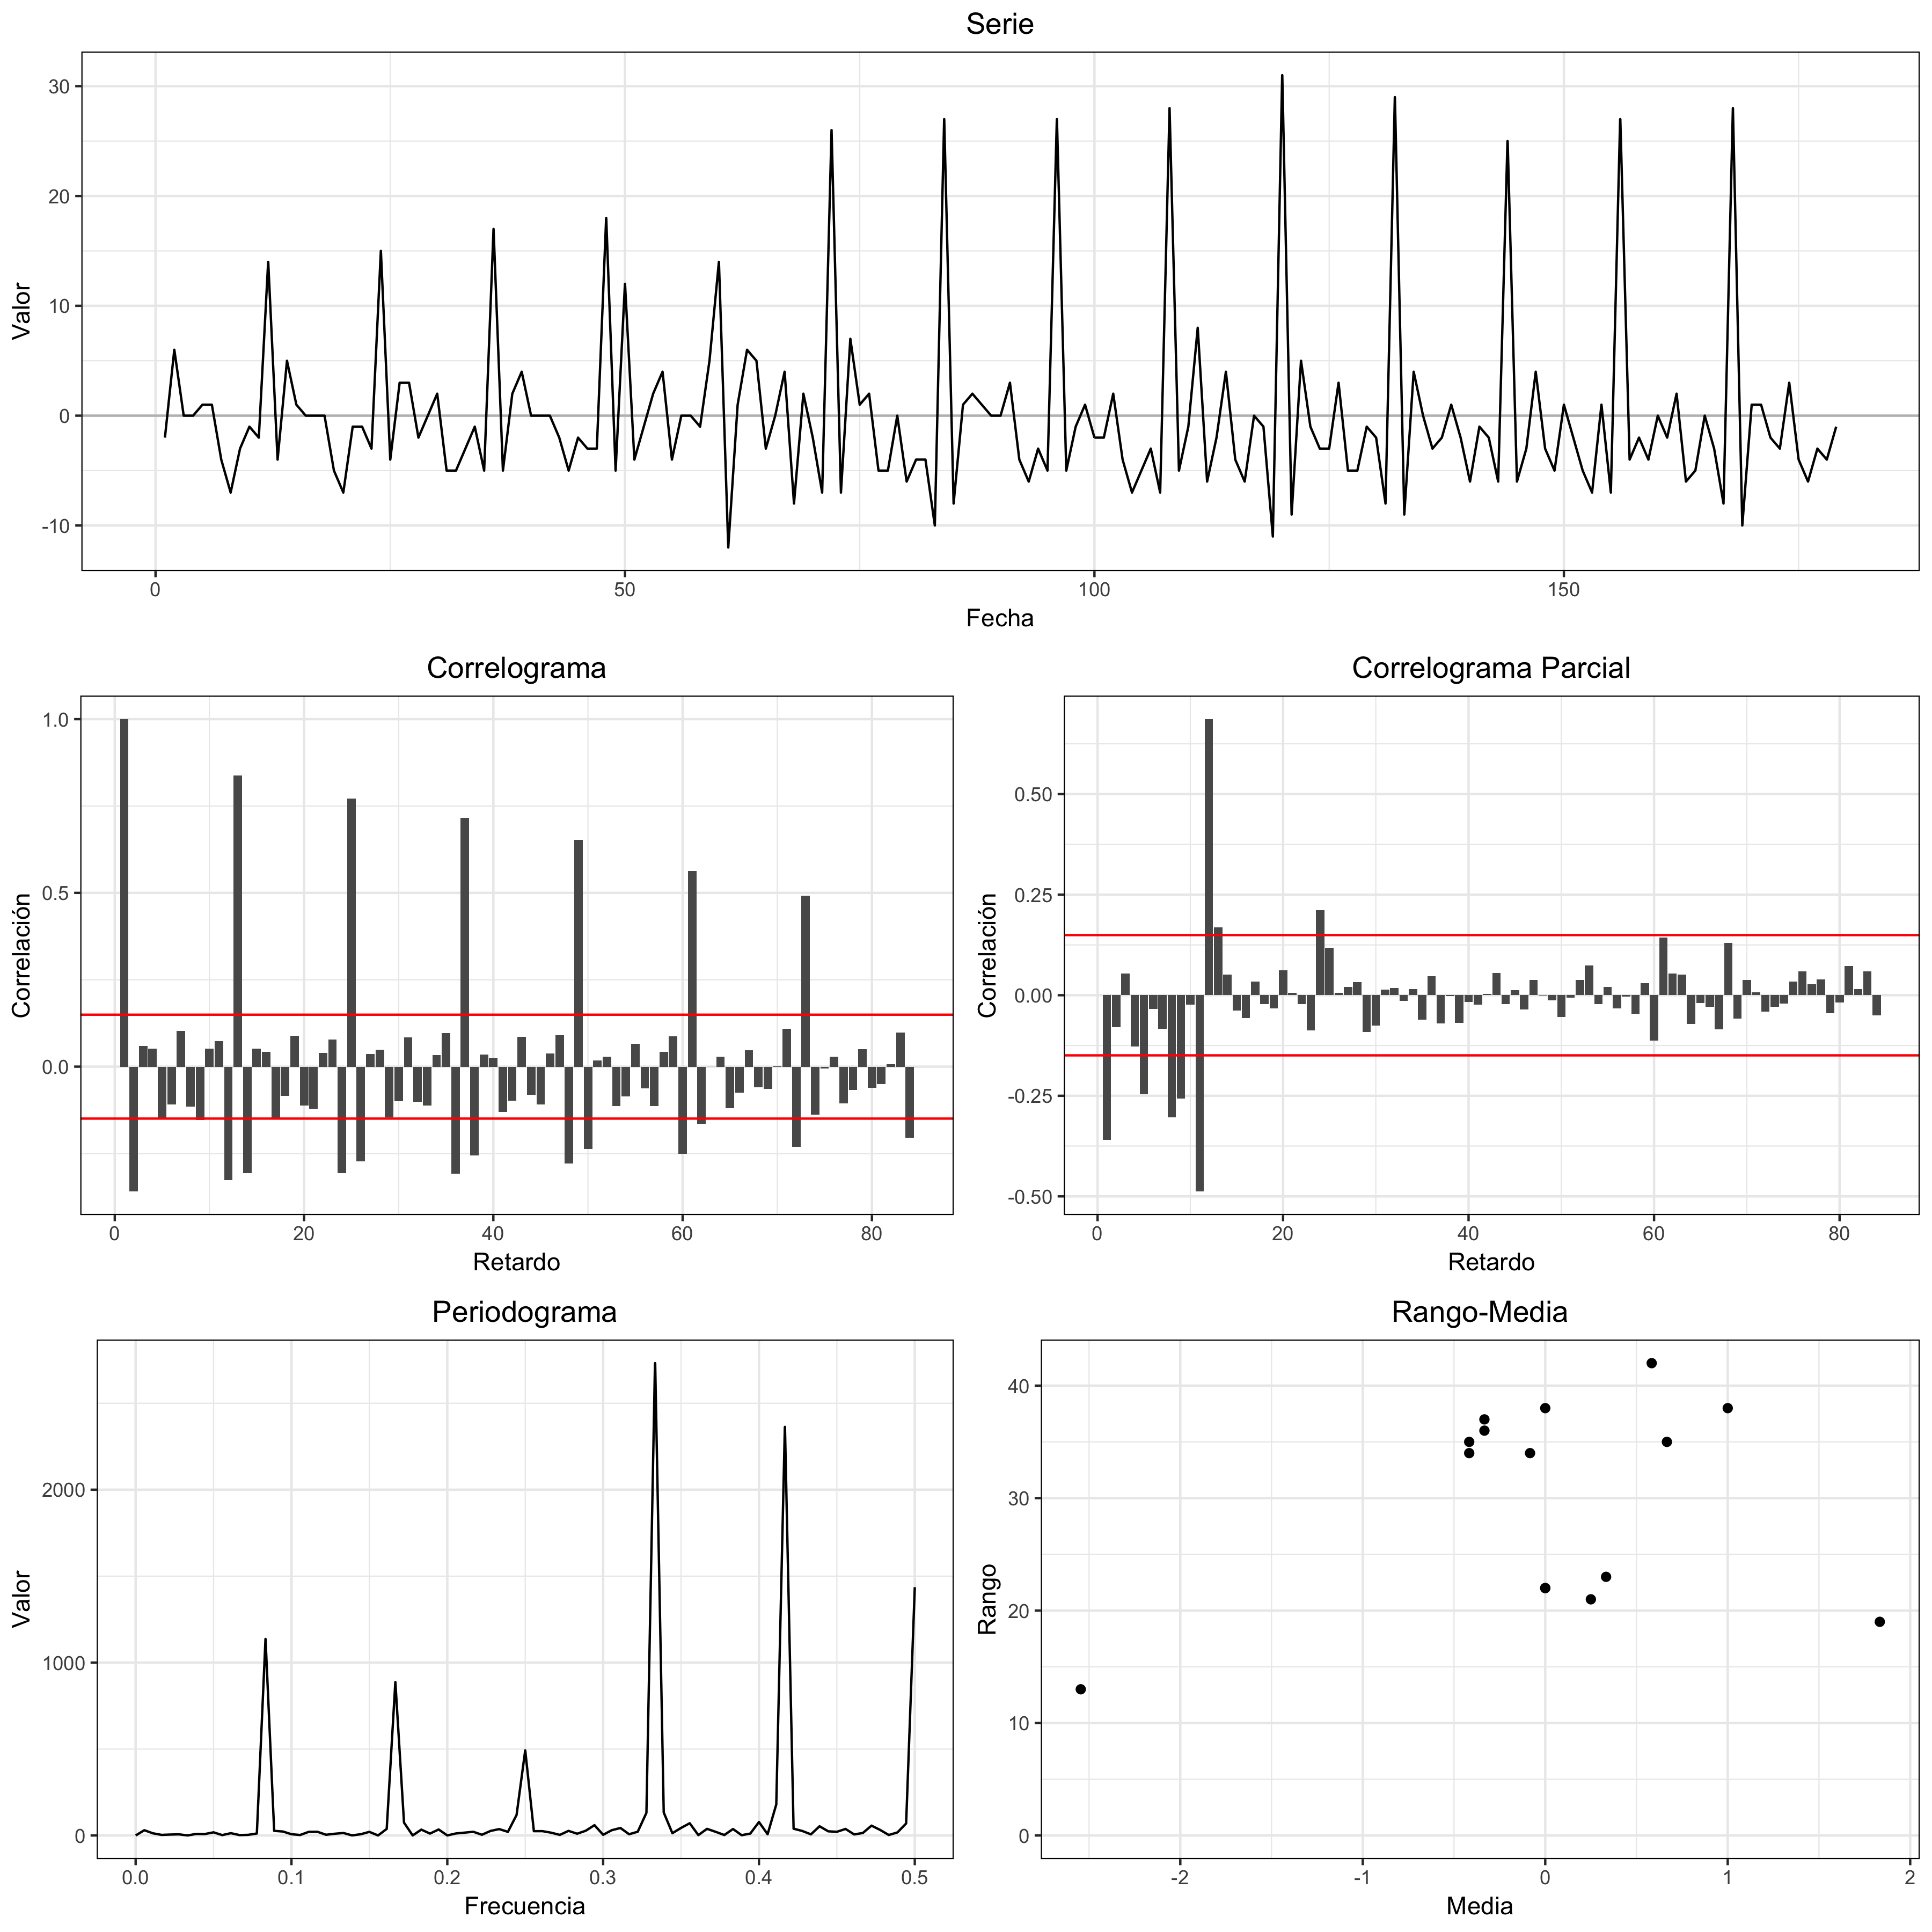
\includegraphics[width=\textwidth,height=\textheight,keepaspectratio]{weightloss-diff-1}
      \caption{[TODO]}
      \label{}
    \end{figure}

    \paragraph{}
    [TODO]

    \begin{figure}
      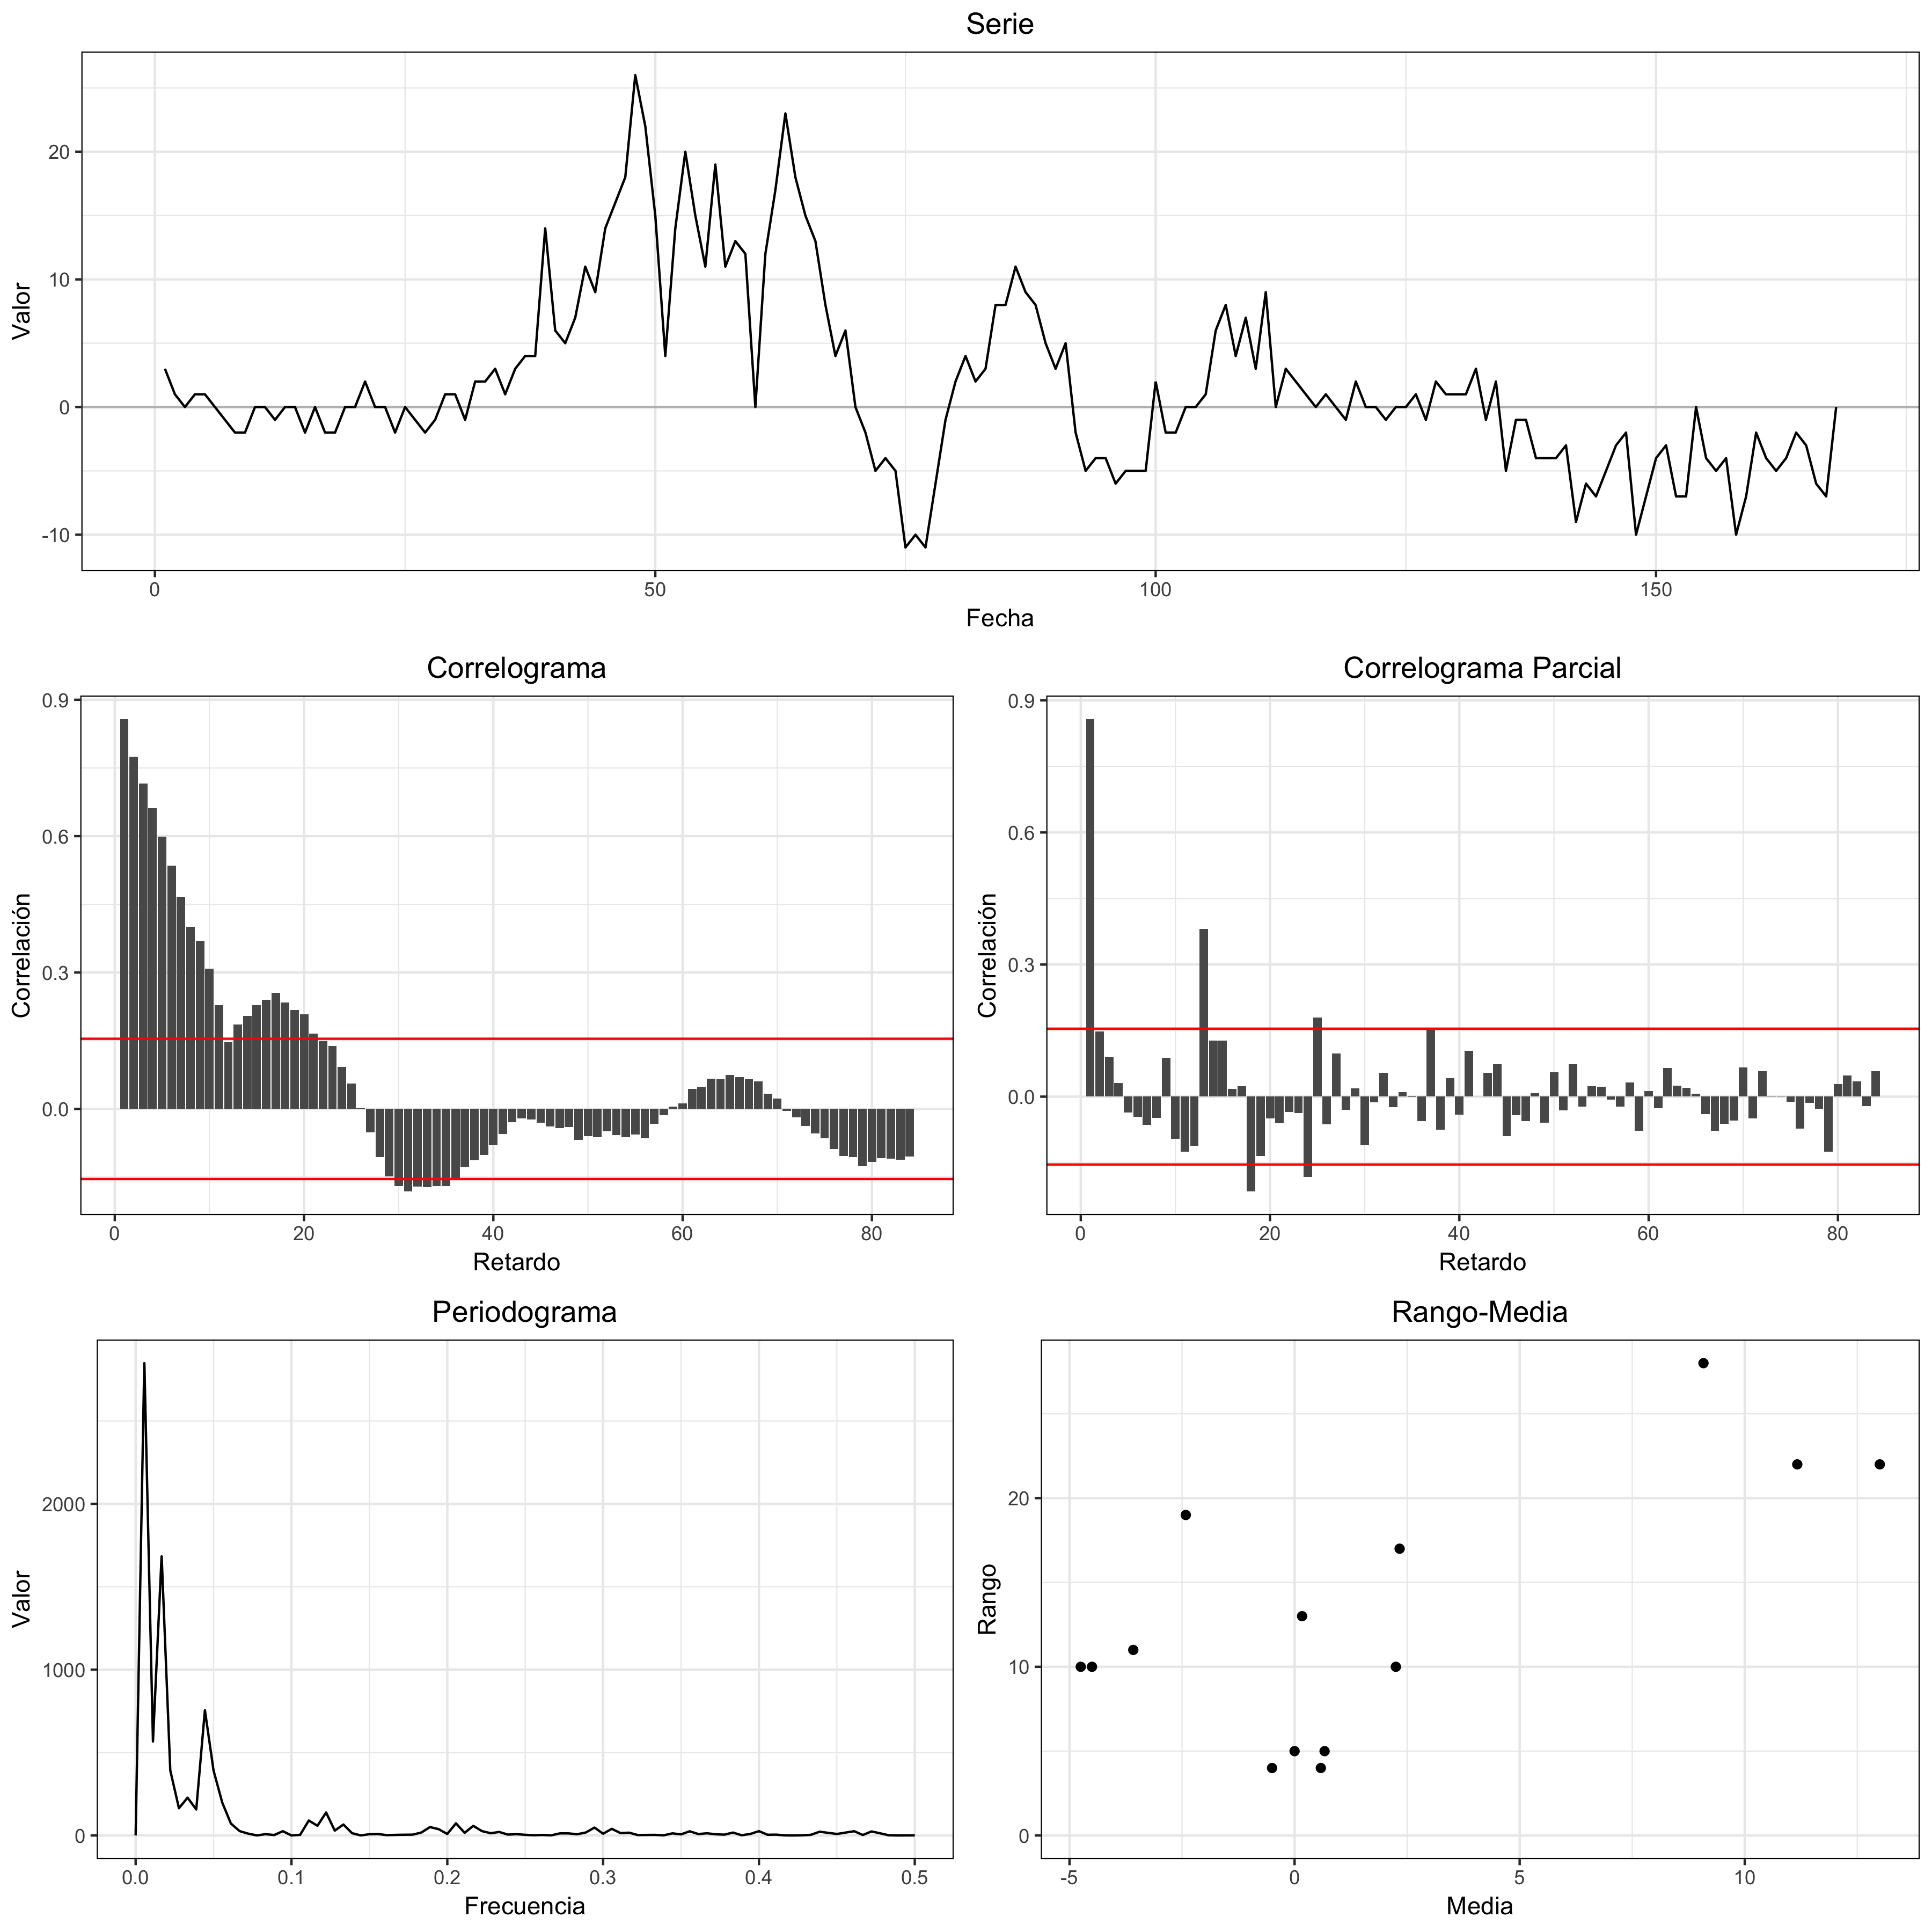
\includegraphics[width=\textwidth,height=\textheight,keepaspectratio]{weightloss-diff-12}
      \caption{[TODO]}
      \label{}
    \end{figure}

    \paragraph{}
    [TODO]

    \begin{figure}
      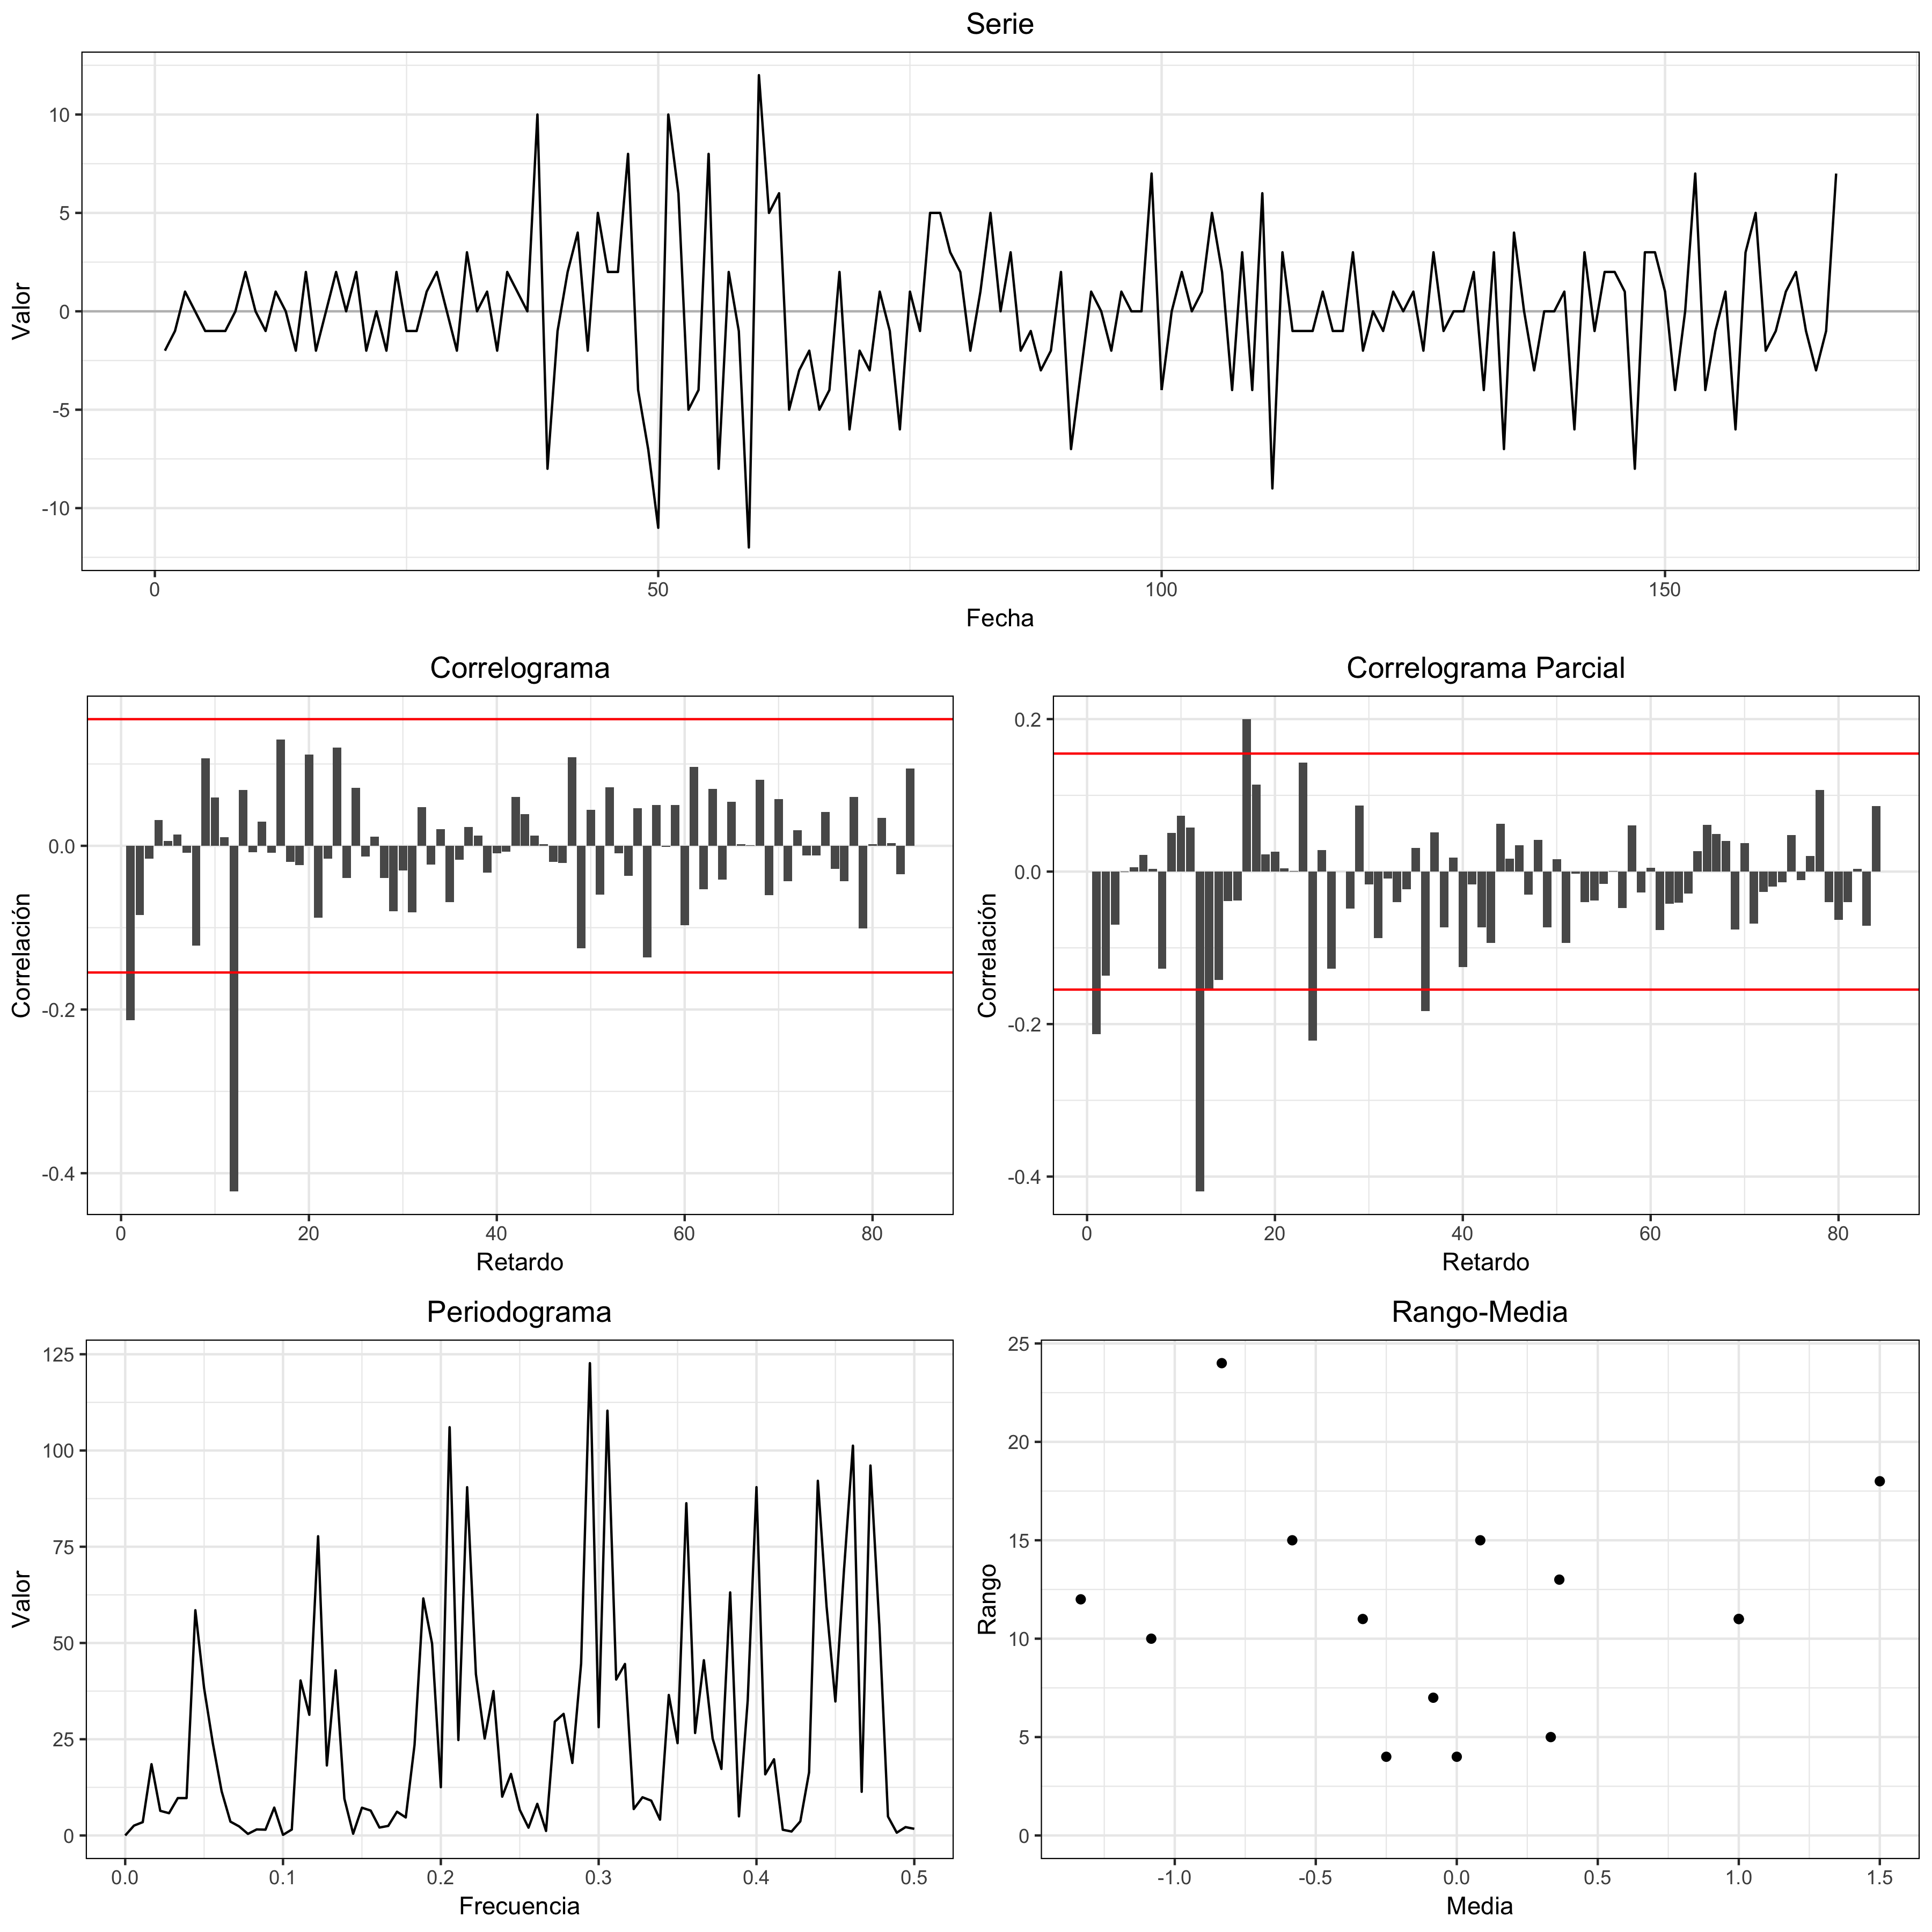
\includegraphics[width=\textwidth,height=\textheight,keepaspectratio]{weightloss-diff-1-12}
      \caption{[TODO]}
      \label{}
    \end{figure}

    \paragraph{}
    [TODO]

  \section{Etapa de estimación y validación}
  \label{sec:2}

    \paragraph{}
    [TODO]

  \section{Comparación de modelos}
  \label{sec:comparison}

    \paragraph{}
    [TODO]

  \section{Predicción}
  \label{sec:prediction}

    \paragraph{}
    [TODO]

  \appendix
  \section{Código Fuente}
  \label{sec:code}

    \paragraph{}
    [TODO]


    \begin{listing}[H]
        \centering
        \inputminted{R}{./res/code/weight-loss.r}
        \caption{[TODO]}
        \label{}
      \end{listing}
\end{document}
